\documentclass[12pt,a4paper]{article}
\usepackage{cmap} % Makes the PDF copiable. See http://tex.stackexchange.com/a/64198/25761
\usepackage[T1]{fontenc}
\usepackage[brazil]{babel}
\usepackage[utf8]{inputenc}
\usepackage{amsmath}
\usepackage{amsfonts}
\usepackage{amssymb}
\usepackage{amsthm}
\usepackage{textcomp} % \degree
\usepackage{gensymb} % \degree
\usepackage[usenames,svgnames,dvipsnames]{xcolor}
\usepackage{hyperref}
\usepackage{multicol}
\usepackage{graphicx}
\usepackage{systeme}
\usepackage[margin=2cm]{geometry}

\hypersetup{
    colorlinks = true,
    allcolors = {blue}
}

\newcommand{\vect}[1]{\overrightarrow{#1}}
\newcommand{\norm}[1]{\left|\left|{#1}\right|\right|}

\newcommand*\tipo{PROVA IV}
\newcommand*\turma{TURMA C}
\newcommand*\disciplina{GAN0001}
\newcommand*\nome{GEOMETRIA ANALÍTICA}
\newcommand*\eu{Helder G. G. de Lima}
\newcommand*\data{26/06/2015}

\author{\eu}
\title{\tipo - \disciplina}
\date{\data}

\begin{document}
\thispagestyle{empty}
\newgeometry{margin=2cm,bottom=0.5cm}
\begin{center}

\includegraphics{udesc_joinville_cabecalho.pdf}
\\ Prof. \eu\footnote{
Este é um material de acesso livre distribuído sob os termos da licença \href{https://creativecommons.org/licenses/by-sa/4.0/deed.pt_BR}{Creative Commons BY-SA 4.0}.}

\noindent\begin{tabular}{l c c r}
  \textbf{\disciplina}
& \textbf{\tipo}
& \textbf{\data}
& \textbf{\turma}
\end{tabular}\vspace{-0.3cm}
\noindent\rule{17cm}{0.01cm}
\end{center}

\noindent Nome do(a) aluno(a): \rule{13cm}{0.01cm}

%\section*{Instruções}
{\footnotesize
\begin{enumerate}
\renewcommand{\theenumi}{\Roman{enumi}}
\item Identifique-se em todas as folhas.
\item Mantenha o celular e os demais equipamentos eletrônicos desligados durante a prova.
\item Justifique cada resposta com cálculos ou argumentos baseados na teoria estudada.
\item Escolha \textsc{\textbf{uma}} questão para \textsc{\textbf{não}} fazer (ela não será corrigida): \rule{3cm}{0.01cm}
\end{enumerate}
}
\section*{Questões}

\begin{enumerate}
\item A equação $r\cos(\theta) = 2$ representa uma curva em coordenadas polares.
\begin{enumerate}
\item (0,5 pontos) Explique se há simetria em relação a algum eixo e em relação à origem
\item (0,5 pontos) Escreva as coordenadas polares de 5 pontos pertencentes à curva
\item (1,0 pontos) Esboce o gráfico (utilize o verso desta folha)
\end{enumerate}

\item (2,0 pontos) Se $r = 12 \cos(\theta)$ é a equação de uma elipse em coordenadas polares, qual é a equação (padrão) em coordenadas cartesianas? E as coordenadas polares do centro?

\item Considere a superfície $\dfrac{(x-2)^2}{4} + (y-1)^2 - \dfrac{(z-3)^2}{9} = 1$.
\begin{enumerate}
\item (0,4 pontos) Qual é o nome da superfície?
\item (1,6 pontos) Descreva (por nome e equação) as interseções da superfície com os planos $x - 6 = 0$ e $z - 6 = 0$.
\end{enumerate}

\item Seja $r(1 + 3 \cos(\phi))(1 - 3\cos(\phi)) = 4$ a equação de uma superfície em coordenadas esféricas.
\begin{enumerate}
\item (1,0 pontos) Qual é a equação da superfície em coordenadas cartesianas?
\item (0,6 pontos) Quais são os pontos de interseção com os eixos coordenados?
\item (0,4 pontos) Qual é o nome da superfície?
\end{enumerate}

\item (2,0 pontos) Determine a equação da superfície esférica que passa pelos pontos $P=(1,0,0)$, $Q=(0,1,0)$ e $R=(0,0,1)$ e cujo centro pertence ao plano $\pi: x-y+z=2$.

\item (2,0 pontos) Esboce a superfície $y + 1 = x^2 + z^2$, explicitando as equações dos traços para os planos $x = 0$, $y=0$ e $z=0$, e as coordenadas dos pontos de interseção com os eixos.
\end{enumerate}

\section*{Lembrete}
\begin{itemize}\footnotesize
\begin{multicols}{2}
\item Coordenadas polares:
$\begin{cases}
x & = r \cos(\theta)\\
y & = r \operatorname{sen}(\theta)\\
r^2 & = x^2 + y^2
\end{cases}$

\item Coordenadas esféricas:
$\begin{cases}
x & = r \operatorname{sen}(\phi) \cos(\theta)\\
y & = r \operatorname{sen}(\phi) \operatorname{sen}(\theta)\\
z & = r \cos(\phi)\\
r^2 & = x^2 + y^2 + z^2
\end{cases}$
\end{multicols}
\end{itemize}

\newpage
\restoregeometry
%\begin{enumerate}
\begin{multicols}{2}
%\renewcommand{\theenumi}{\alph{enumi}}%
%\item
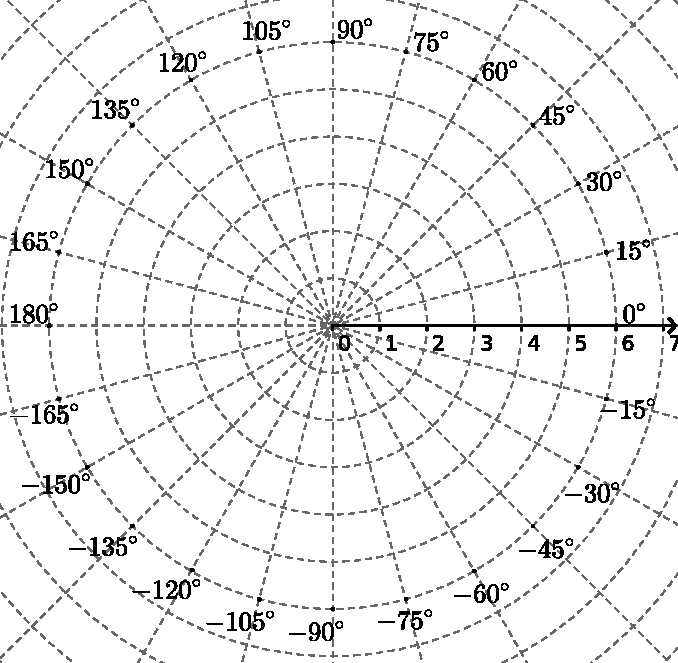
\includegraphics[width=7.5cm]{img/prova-4-pro-malha-1}
\vspace{2em}
%\item
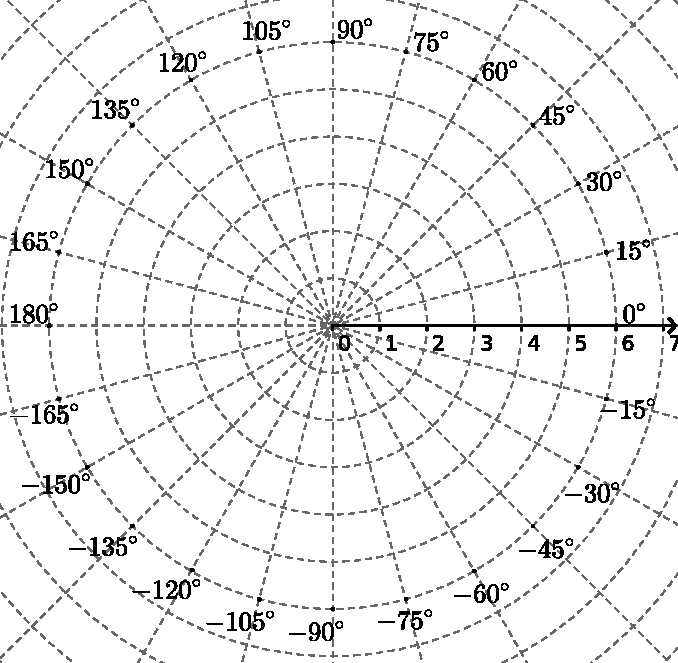
\includegraphics[width=7.5cm]{img/prova-4-pro-malha-1}
\end{multicols}
%\item

\includegraphics[width=16cm]{img/prova-4-pro-malha-2}

\vspace{2em}

\includegraphics[width=16cm]{img/prova-4-pro-malha-2}
%\end{enumerate}

%\newpage
%\section*{Respostas e observações}
\end{document}
